\selectlanguage{ngerman}
\subsection{Sensor}\label{ch:Umsetzung_Sensor}
% - Objekterkennung auf Frames: vortrainierte Modelle
% - Schwierigkeit: Nicht nur Erkennung einzelner Objekte nötig, sondern Erkennung des Rein- und Rausfahrens der Autos
%     --> zwei Implementierungen, Verweis auf Tests

Die Komponente, welche erkennt, wie viele Autos den Parkplatz befahren und verlassen, wird in dieser Arbeit Sensor genannt, besteht aus einem Mini-Computer und einer Kamera.
Für die konkrete Anwendung (siehe Kapitel~\ref{ch:Test}) wurde ein Raspberry Pi Model B+ und ein Pi Camera Module v2.1 verwendet.
Auf diesem läuft kontinuierlich eine Software, welche den Kamera-Input verarbeitet und hieraus die rein- und rausfahrenden Autos erkennt.
Die Herausforderung besteht darin, nicht nur die Erkennung einzelner Fahrzeuge in den einzelnen Frames zu ermöglichen, sondern auch das Ein- und Ausfahren der Fahrzeuge zu identifizieren.
Um dieses Problem zu lösen, werden zwei verschiedene Implementierungen, welche im Folgenden erklärt werden, entwickelt und in Kapitel~\ref{ch:Test} getestet.

\subsubsection{Variante 0: einfache Objekterkennung}\label{ch:Sensor_v0}
% - sehr performant
% - viel zu ungenau
Zunächst wird versucht, eine Objekterkennung mit dem OpenCV-Framework umzusetzen.
Das Verfahren verwendet Computer-Vision-Techniken wie Hintergrundsubtraktion und Konturen\-erkennung, um Fahrzeuge in einem Video zu erkennen und zu zählen.
Dabei werden Bewegungsunterschiede zwischen Frames erkannt und die Konturen bewegter Objekte identifiziert, um potenzielle Fahrzeuge zu identifizieren.
Die Anzahl der Fahrzeuge wird basierend auf der Position der Konturzentren ermittelt.
Nach den ersten Tests stellt sich das Verfahren allerdings als unbrauchbar heraus.
Das Verfahren ist zwar sehr performant, sodass bis zu 30 Bilder pro Sekunde verarbeitet werden können, die Genauigkeit ist für die Umsetzung des Projektes jedoch zu gering.
Teilweise werden einzelne Fahrzeuge als mehrere gezählt.
Weiterhin gibt es mehrere Objekte und Personen, die von dieser Methode fälschlicherweise als Fahrzeug erkannt werden.
Deshalb wird diese Variante nicht weiter verfolgt und verbessert.

\subsubsection{Variante 1: Richtung des Bewegungsvektors}\label{ch:Sensor_v1}
% - Grundidee: Erkennen in welche Richtung im Bild (oben oder unten) Auto fährt
% - Vorgehen: 
%     - Rechtecke (Eckkoordinaten) der Autos durch Objekterkennung
%     - Berechnung der Mittelpunkte
%     - Berechnung der Bewegungsrichtung 
%         - Für jeden Punkt im aktuellen Frame werden die Distanzen zu den Punkten des vorherigen Frames errechnet
%         - Der Punkt mit der jeweils kürzesten Distanz wird ausgewählt und mit diesem der Bewegungsvektor errechnet. Falls bereits passender früherer Bewegungsvektor vorhanden, wird Aufaddiert, da nur Gesamtergebnis wichtig  
%         - Punkte des vorherigen Frames, die für keinen aktuellen Punkt die kürzeste Verbindung waren (weil jetzt weniger Autos im Bild), werden gesucht und deren Bewegungsvektor für Zählung verwendet 
%     - Anhand der Richtung der y Koordinate es Vektors die Richtung (oben/unten) des Autos bestimmen 
%     - API Aufruf

Um Autos nur einmal zu erkennen wurde ein anderer Ansatz verfolgt, der im Folgenden beschrieben wird.

Die Grundidee des Algorithmus besteht darin, die Richtung zu ermitteln, in die ein Fahrzeug im Bild fährt.
Hierbei wurde die vereinfachte Annahme getroffen, dass Autos, die sich im Kamerabild nach oben bewegen, aus dem Parkhaus fahren, während Autos, die sich nach unten bewegen, in das Parkhaus hinein fahren.
Diese Annahme gilt nur, wenn die Kamera von oben aus dem Inneren des Parkhauses die Ein- und Ausfahrt filmt.
Andernfalls müssten die Richtungen entsprechend angepasst werden.

Zunächst werden die Fahrzeuge in den einzelnen Frames mithilfe von einem vortrainierten Modell, konkret YOLOv5~\cite{yolov5}, für die Objekterkennung identifiziert.
Die Eckkoordinaten der erkannten Fahrzeuge werden dann verwendet, um die Mittelpunkte der Fahrzeuge zu berechnen.
Die Berechnung der Bewegungsrichtung auf Basis der Mittelpunkte erfolgt in mehreren Schritten.
Hierfür werden für jeden Punkt im aktuellen Frame die Distanzen zu den Punkten des vorherigen Frames ermittelt.
Hiervon wird jeweils der Punkt mit der kürzesten Distanz ausgewählt und der Bewegungsvektor zwischen den zwei Punkten berechnet.
Sollte bereits ein passender Bewegungsvektor für den Punkt aus vorherigen Frames vorhanden sein, wird dieser Vektor aufaddiert, da nur das Gesamtergebnis relevant ist.
Der hieraus resultierende Vektor zeigt also von der ersten Sichtung des Autos zu seiner aktuellen Position und ist in Abbildung~\ref{fig:Variante1} blau dargestellt.

\begin{figure}[h]
	\myImagePos{}
	\includegraphics[width=\myImageWidth]{Bilder/Methode2_Beispiel.png}
	\caption[Fahrzeugerkennung Variante 1 Beispiel]{Beispiel der Fahrzeugerkennung mit Variante 1 (Quelle: eigene Darstellung)}
	\label{fig:Variante1}
\end{figure}

Zur Zählung werden die errechneten Bewegungsvektoren verwendet, wenn das entsprechende Auto das Kamerasichtfeld verlassen hat.
Das ist der Fall, wenn Punkte des vorherigen Frames für keinen Punkt im aktuellen Frame die kürzeste Verbindung darstellten, weil jetzt weniger Autos im Bild zu sehen sind als im vorherigen Frame.
In diesem Fall werden die zuvor berechneten Bewegungsvektoren der nicht zugeordneten Punkte für die Zählung verwendet.
Selbst wenn zwischen den Frames ein neues Auto in den Bildausschnitt fährt, während ein anderes ihn verlässt, stellt dies kein Problem dar, weil dies aufgrund eines Schwellwerts nur für Autos passieren kann, die in entgegengesetzte Richtungen fahren und sich die aufaddierten Bewegungsvektoren folglich ausgleichen, sodass der Zählerwert ebenso unverändert bleibt.
In Abbildung~\ref{fig:Variante1} ist in Weiß der Vektor des vorherigen Autos zu sehen.

Die Richtung des Fahrzeugs wird anhand der y-Koordinate des Bewegungsvektors bestimmt.
Wenn die y-Koordinate des Vektors positiv ist, fährt das Fahrzeug nach unten, andernfalls fährt es nach oben, was durch die bereits erwähnte Vereinfachung einen Rückschluss auf die tatsächliche Fahrtrichtung des Autos ermöglicht.
Der interne Zähler des Sensors wird daraufhin entsprechend inkrementiert oder dekrementiert und über eine HTTP PUT-Request im, in Kapitel~\ref{ch:Umsetzung_Server} beschrieben Format, als JSON an den Server übertragen.

\subsubsection{Variante 2: Überschreiten einer Linie}\label{ch:Sensor_v2}
% - Grundidee: Einteilen des Videos in zwei Bereiche (horizontal - z. B. Einfahrt des Parkhaus)- bei Änderung des Bereichs -> hoch- oder runterzählen
% - Vorgehen:
% 	- Mittelpunkt der Objekterkennung
%	- jedes Auto mit ID versehen
%	- schauen in welchem Bereich sich ID befindet
% 	- Bei Änderung des Bereichs hoch bzw. runterzählen
%		- API Aufruf

Die grundlegende Idee des Algorithmus besteht darin, Fahrzeuge in den Frames eines Videos mithilfe von YOLOv8 zu identifizieren und dann ihre Bewegung in Bezug auf eine festgelegte Linie zu verfolgen, um die Fahrtrichtung zu bestimmen.
Die Linie wird dabei horizontal über der Einfahrt des Parkhauses festgelegt, wie dies in Abbildung \ref{fig:Variante2} zu sehen ist.
Somit wird das Bild in zwei Zonen geteilt.
Ändert sich die Position eines Autos von der oberen in die untere Zone des Bildes, so wird die Anzeige der freien Parkplätze um eins verringert, da sich nun ein Auto mehr im Parkhaus befindet.
Geschieht eine Änderung der Position von unten nach oben, so wird die Anzeige um eins erhöht.

\begin{figure}[h]
	\myImagePos{}
	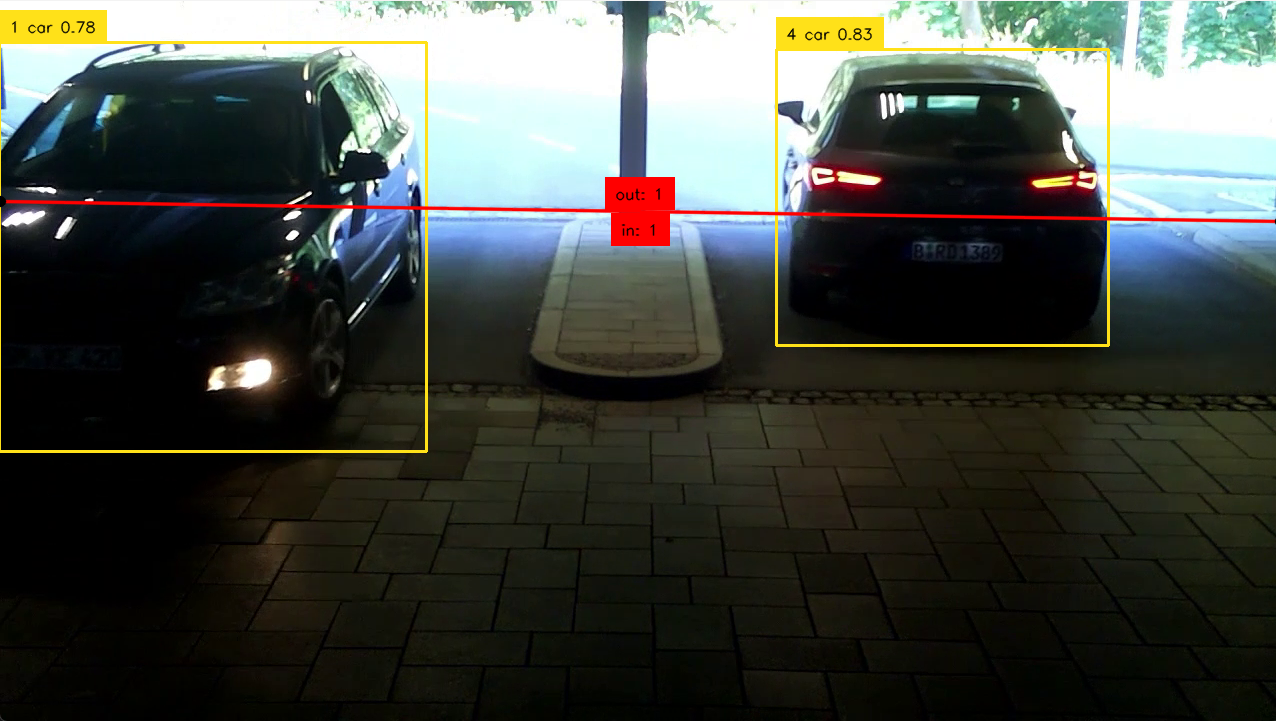
\includegraphics[width=\myImageWidth]{Bilder/Method3_Beispiel.png}
	\caption[Fahrzeugerkennung Variante 2 Beispiel]{Beispiel der Fahrzeugerkennung mit Variante 2 (Quelle: eigene Darstellung)}
	\label{fig:Variante2}
\end{figure}

Es wird YOLOv8 eingesetzt, um die Fahrzeuge in den einzelnen Frames des Videos zu erkennen.
Der Vorteil des Frameworks ist es, dass es Objekten IDs zuordnen kann.
Somit ist eine eindeutige Zuordnung eines Autos über mehrere Frames hinweg möglich.
Die Zuordnung einer ID zu einem konkreten Auto über eine gewisse Dauer geschieht über verschiedene Merkmale des Objektes, wie die Eckpunkte der Objekterkennung, die Geschwindigkeit des Autos oder die Veränderung der Zuverlässigkeitswerte des Algorithmus.
Die erkannten Fahrzeuge werden durch ihre Eckkoordinaten repräsentiert.
Der daraus errechnete Mittelpunkt gibt Aufschluss über die Position des Fahrzeuges.

Der Algorithmus nutzt die erfassten Zählerwerte, um die aktuelle Auslastung des Parkhauses an einen Server zu übertragen.
Dazu wird eine HTTP PUT-Request im JSON-Format verwendet, um die Zählerwerte an den Server zu senden und die Fahrzeugbewegungen zu protokollieren.